\documentclass[letter]{article} 
\addtolength{\hoffset}{-2.25cm}
\addtolength{\textwidth}{4.5cm}
\addtolength{\voffset}{-3.25cm}
\addtolength{\textheight}{5cm}
\setlength{\parskip}{0pt}
\setlength{\parindent}{0in}

\usepackage[square,sort,comma,numbers]{natbib}
\usepackage{blindtext} % Package to generate dummy text
\usepackage{charter} % Use the Charter font
\usepackage[utf8]{inputenc} % Use UTF-8 encoding
\usepackage{microtype} % Slightly tweak font spacing for aesthetics
\usepackage{amsthm, amsmath, amssymb, setspace} % Mathematical typesetting
\usepackage{float} % Improved interface for floating objects
\usepackage{hyperref} % For hyperlinks in the PDF
\usepackage{graphicx, multicol} % Enhanced support for graphics
\usepackage{xcolor} % Driver-independent color extensions
\usepackage{pseudocode} % Environment for specifying algorithms in a natural way
\usepackage[ddmmyyyy]{datetime} % Uses YEAR-MONTH-DAY format for dates
\usepackage[spanish, activeacute, es-lcroman]{babel}

\usepackage{fancyhdr} % Headers and footers
\pagestyle{fancy} % All pages have headers and footers
\fancyhead{}\renewcommand{\headrulewidth}{0pt} % Blank out the default header
\fancyfoot[L]{} % Custom footer text
\fancyfoot[C]{} % Custom footer text
\fancyfoot[R]{\thepage} % Custom footer text
\newcommand{\note}[1]{\marginpar{\scriptsize \textcolor{red}{#1}}} % Enables comments in red on margin

\makeatletter
\renewcommand\subsection{\@startsection{subsection}{3}{\z@}%
                                     {-3.25ex\@plus -1ex \@minus -.2ex}%
                                     {-1.5ex \@plus -.2ex}% Formerly 1.5ex \@plus .2ex
                                     {\normalfont\normalsize\bfseries}}
\makeatother

\usepackage{listings}
\lstloadlanguages{[5.2]Mathematica}

\usepackage{enumerate}

\usepackage{subcaption}

\usepackage{dsfont}

\usepackage{wrapfig}

\usepackage{enumitem}

\usepackage{cancel}

\usepackage{booktabs}

%----------------------------------------------------------------------------------------


%-------------------------------
%	TITLE VARIABLES (identify your work!)
%-------------------------------

\newcommand{\firstname}{Nicolas Maldonado Baracaldo}
\newcommand{\firstid}{201423809}
\newcommand{\firstemail}{n.maldonado10@uniandes.edu.co}

\begin{document}

%-------------------------------
%	TITLE SECTION (do not modify unless you really need to)
%-------------------------------
\fancyhead[C]{}
\hrule \medskip
\begin{minipage}{0.295\textwidth} 
\raggedright
\footnotesize
\firstname \hfill\\ 
\firstid \hfill\\ 
\firstemail \hfill\\
\end{minipage}
\begin{minipage}{0.4\textwidth} 
\centering 
\large 
Introducción a los Modelos Matemáticos en Gestión Financiera (MATE2714)\\ 
\normalsize
Rene Joaquin Meziat Velez\\
Proyecto 3\\ 
\end{minipage}
\begin{minipage}{0.295\textwidth} 
\raggedleft
\today\hfill\\
\end{minipage}
\medskip\hrule 
\bigskip

\newcommand{\mathsym}[1]{{}}
\newcommand{\unicode}[1]{{}}

%-------------------------------
%	ASSIGNMENT CONTENT (add your responses)
%-------------------------------

\bigskip

\begin{enumerate}

\item \emph{Elabore un programa de computadora que simule el comportamiento de un modelo de árbol binomial para precios de activos. Éste debe recibir como parámetros el número de periodos, el factor de valorización, el factor de depreciación, sus respectivas probabilidades y un precio inicial. El programa debe mostrar la evolución del precio del activo en los diferentes periodos.}

\medskip

\textbf{\textit{Sol.}} Se escribió en \texttt{Wolfram Mathematica 12.1} la siguiente función que genera contenido dinámico

\begin{doublespace}
\noindent\(\pmb{\text{Manipulate}[S=\{\text{S1}\};\text{SeedRandom}[2248];}\\
\pmb{\text{For}[n=1,n<T,n\text{++},\text{ran}=\text{RandomVariate}[\text{BernoulliDistribution}[p]];}\\
\pmb{\text{If}[\text{ran}==1,\text{AppendTo}[S,S[[-1]]u],\text{AppendTo}[S,S[[-1]]d]]];}\\
\pmb{\text{ListLinePlot}\left[S,\text{Axes}\to \text{False},\text{Frame}\to \text{True},\text{FrameLabel}\to \left\{\text{``Periodo (n)''},\text{``Precio (}S_n\text{)''}\right\},\right.}\\
\pmb{\left.\text{ImageSize}\to \text{Full},\text{PlotRange}\to \text{All}\right],}\\
\pmb{\left\{\left\{\text{S1},4,\text{``}S_1\text{(Precio Inicial)''}\right\}\right\},\{\{p,0.5,\text{{``}p (Probabilidad de Valorizaci{\' o}n){''}}\},0.01,0.99\},}\\
\pmb{\{\{u,2,\text{{``}u (Factor de Valorizaci{\' o}n){''}}\}\},\left\{\left\{d,\frac{1}{u},\text{{``}d
(Factor de Depreciaci{\' o}n){''}}\right\},0,u\right\},}\\
\pmb{\{\{T,10,\text{{``}N (N{\' u}mero de Periodos){''}}\},10,1000,1\},\text{TrackedSymbols}:\to \{\text{S1},p,u,d,T\}]}\)
\end{doublespace}

cuyo resultado es una ventana que permite modificar todos los parámetros y genera la gráfica resultante de dicho proceso como puede observarse en la figura \ref{fig:sim1}

\begin{figure}[h!]
    \centering
    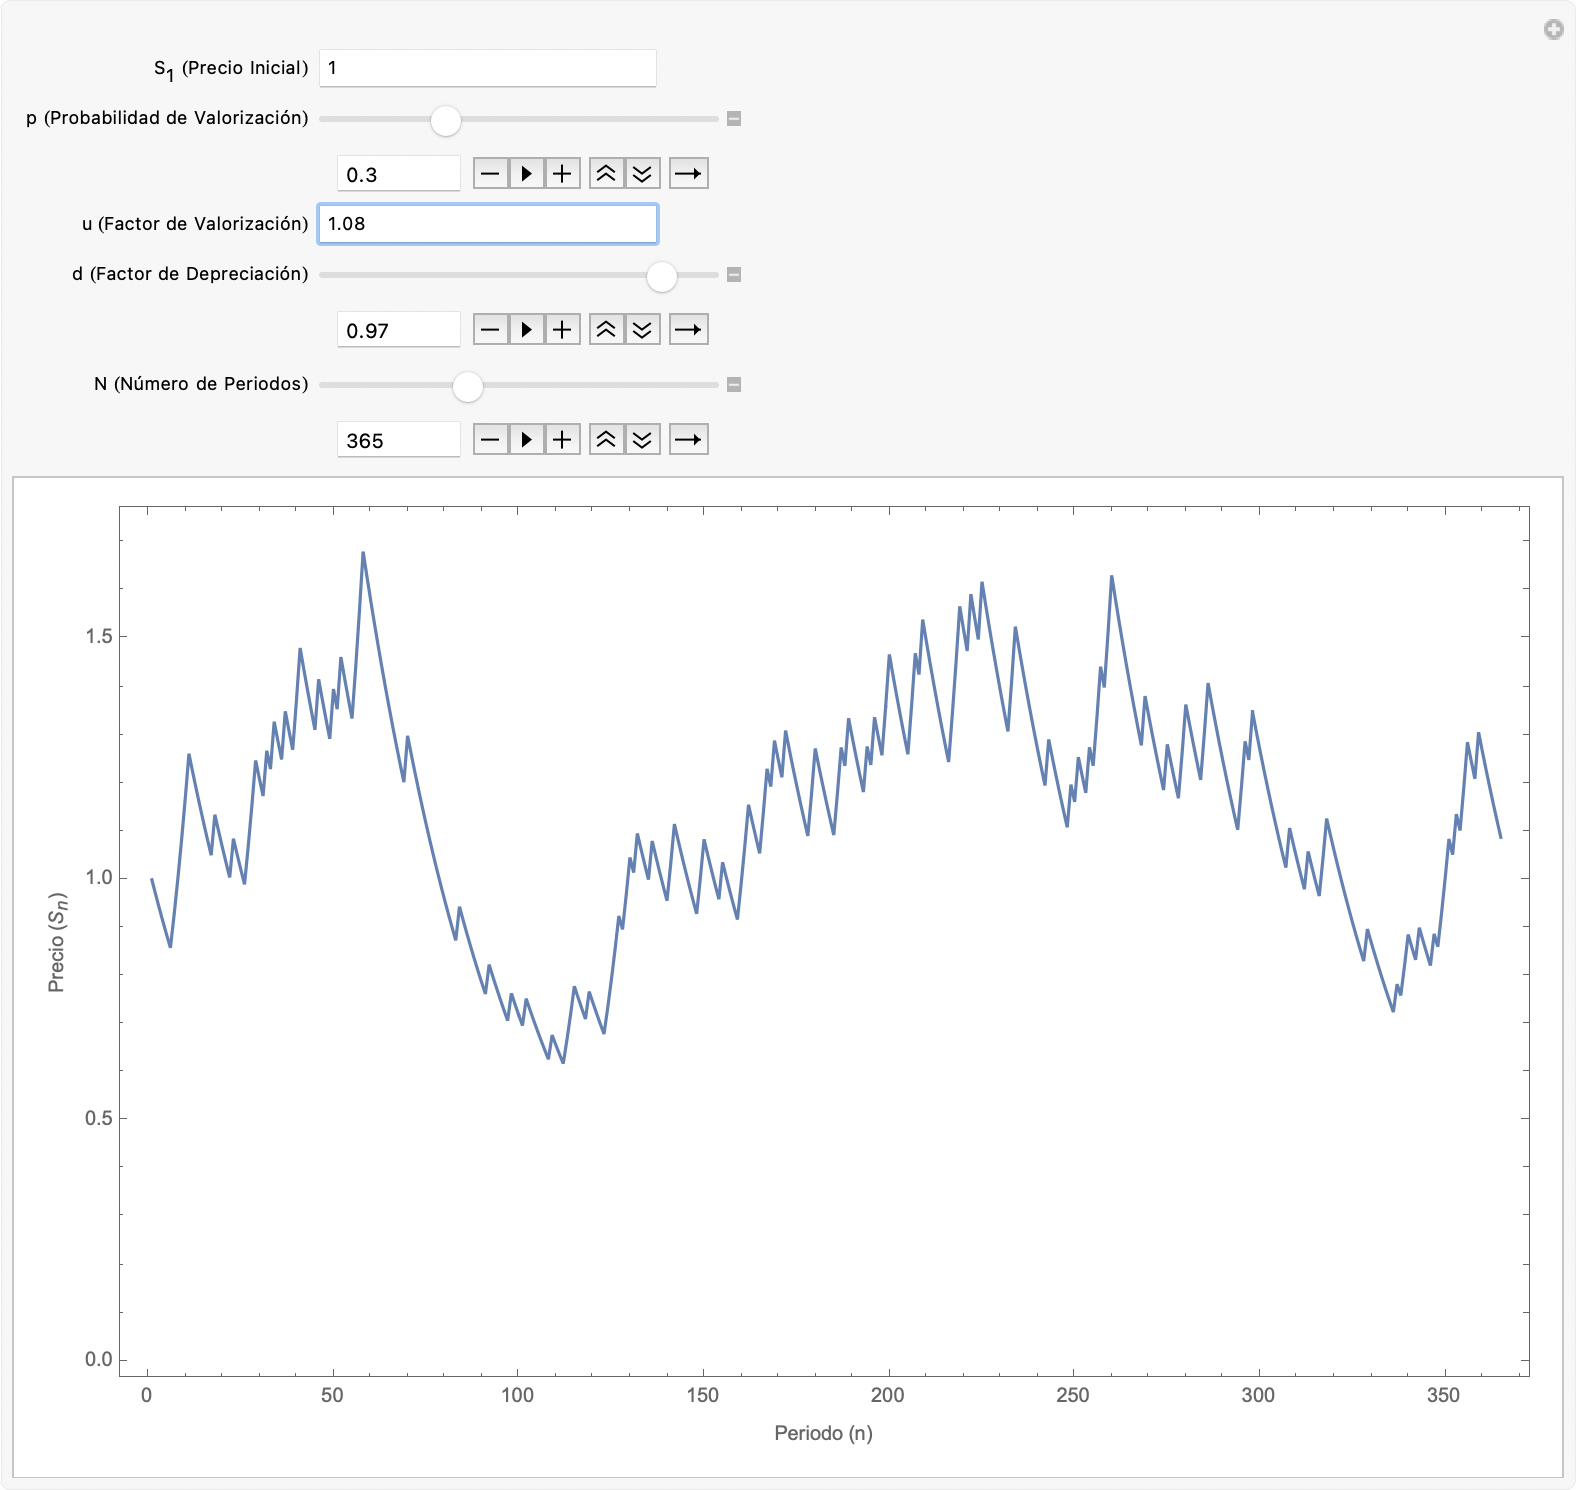
\includegraphics[width=0.5\textwidth]{sim1.png}
    \caption{Visualización del modelo de árbol binomial. Puede verse cómo los distintos parámetros son modificables por el usuario así como la gráfica que se genera.}
    \label{fig:sim1}
\end{figure}

\newpage

\item \emph{Elabore un programa como el anterior, de manera que el usuario introduzca la tasa de interés y los factores de valorización y depreciación. Con ellos el computador debe realizar la simulación empleando la probabilidad de riesgo neutral del modelo. Evidentemente su programa debe rechazar datos que no correspondan a la condición de no arbitraje.}

\medskip

\textbf{\textit{Sol.}} Se escribió en \texttt{Wolfram Mathematica 12.1} la siguiente función que genera contenido dinámico

\begin{doublespace}
\noindent\(\pmb{\text{Manipulate}[\text{If}[d<1+r<u,S=\{\text{S1}\};p=\frac{1+r-d}{u-d};\text{SeedRandom}[2248];}\\
\pmb{\text{For}[n=1,n<T,n\text{++},\text{ran}=\text{RandomVariate}[\text{BernoulliDistribution}[p]];}\\
\pmb{\text{If}[\text{ran}==1,\text{AppendTo}[S,S[[-1]]u],\text{AppendTo}[S,S[[-1]]d]]];}\\
\pmb{\text{ListLinePlot}\left[S,\text{Axes}\to \text{False},\text{Frame}\to \text{True},\text{FrameLabel}\to \left\{\text{{``}Periodo (n){''}},\text{``Precio
(}S_n\text{)''}\right\},\right.\left.\text{ImageSize}\to \text{Full}\right],}\\
\pmb{\text{Catch}[\text{Throw}[\text{{``}Los par{\' a}metros introducidos no corresponden a la condici{\' o}n de no arbitraje{''}}]]],}\\
\pmb{\left\{\left\{\text{S1},4,\text{``}S_1\text{
(Precio Inicial)''}\right\}\right\},\{\{r,0.25,\text{{``}r (Tasa de Inter{\' e}s){''}}\}\},}\\
\pmb{\{\{u,2,\text{{``}u (Factor de Valorizaci{\' o}n){''}}\}\},\left\{\left\{d,\frac{1}{u},\text{{``}d
(Factor de Depreciaci{\' o}n){''}}\right\},0,u\right\},}\\
\pmb{\{\{T,10,\text{{``}N (N{\' u}mero de Periodos){''}}\},10,1000,1\},\text{TrackedSymbols}:\to \{\text{S1},u,d,T\}]}\)
\end{doublespace}

cuyo resultado es una ventana que permite modificar todos los parámetros y genera la gráfica resultante de dicho proceso como puede observarse en la figura \ref{fig:sim2}, además arroja un mensaje cuando los parámetros ingresados no corresponden con la condición de no arbitraje como puede observarse en la figura \ref{fig:sim2arb}

\begin{figure}[h!]
    \centering
    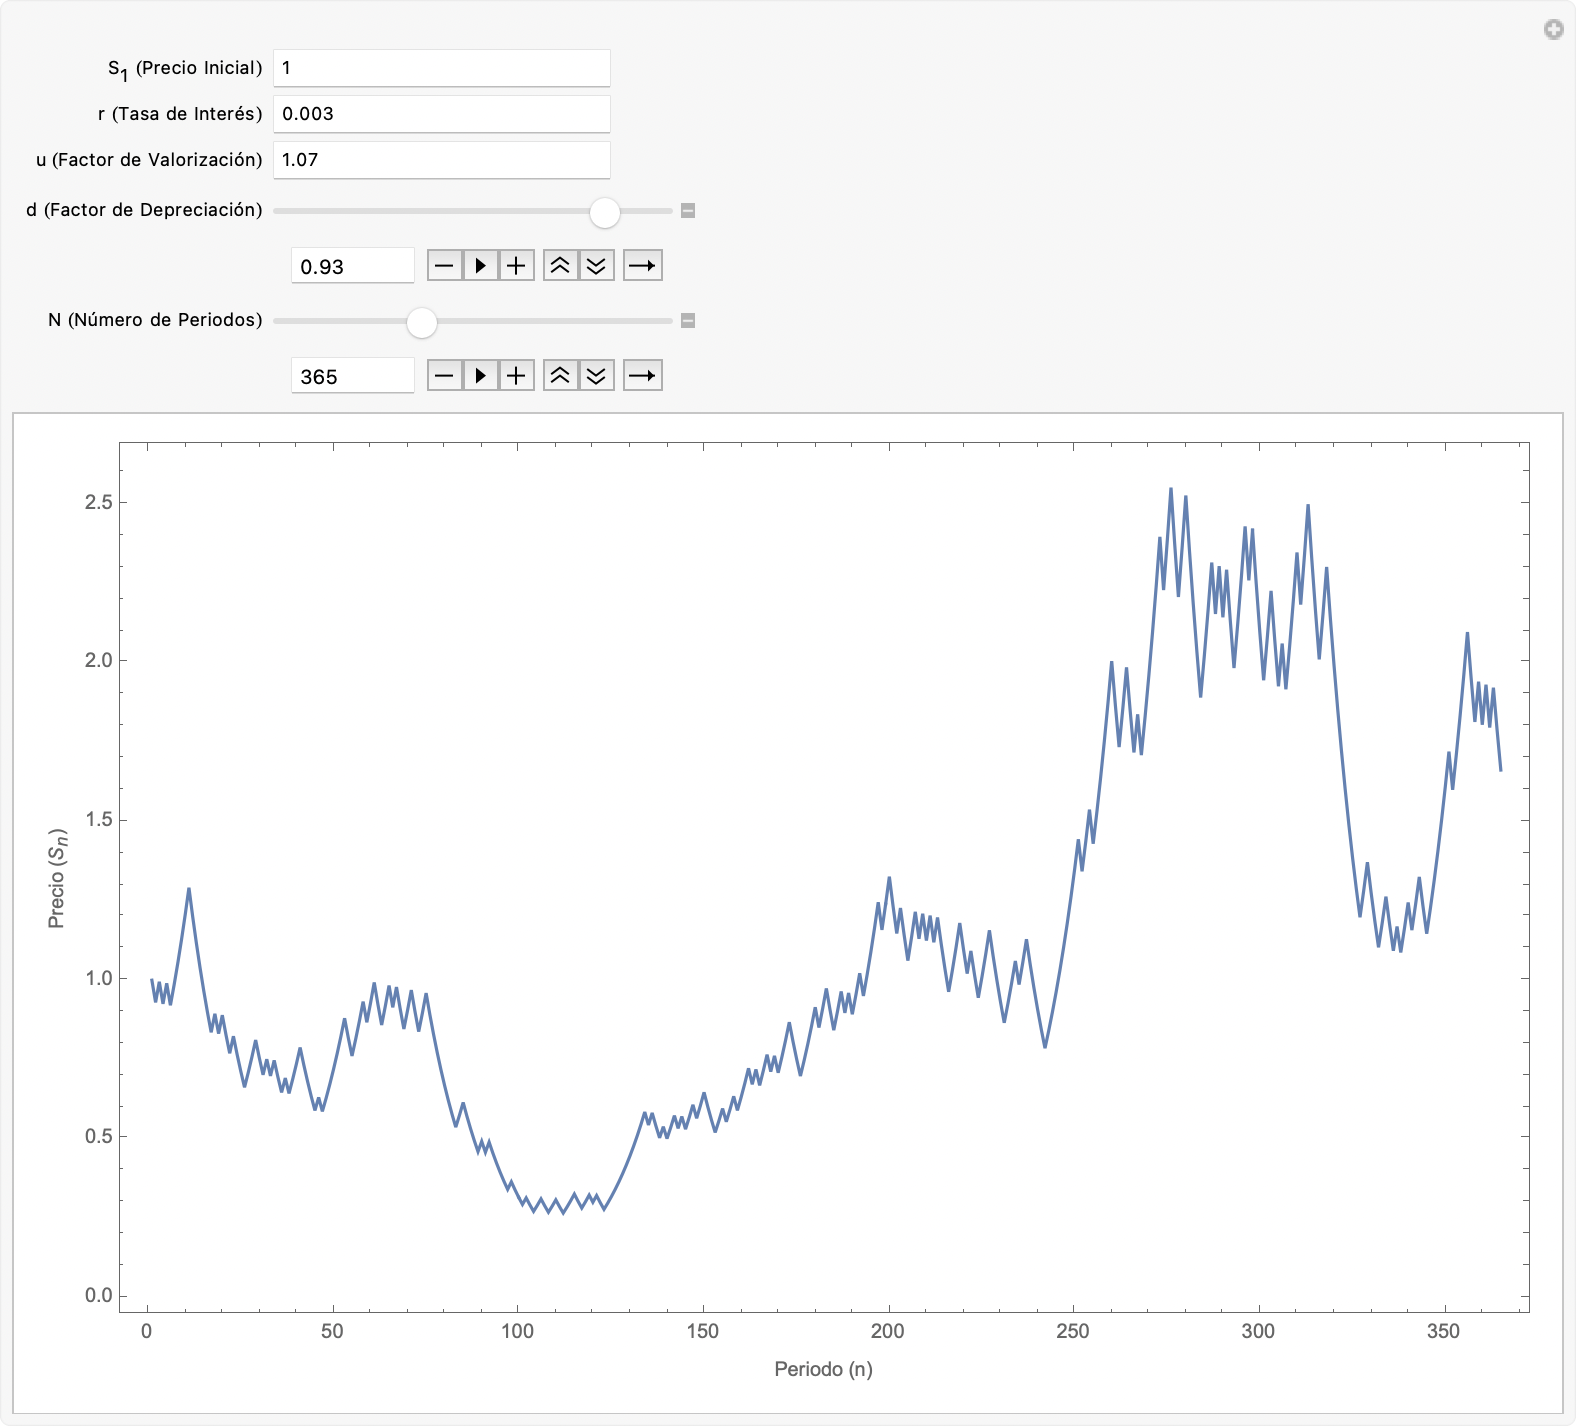
\includegraphics[width=0.5\textwidth]{sim2.png}
    \caption{Visualización del modelo de árbol binomial con probabilidad de riesgo neutral. Puede verse cómo los distintos parámetros son modificables por el usuario así como la gráfica que se genera.}
    \label{fig:sim2}
\end{figure}

\begin{figure}[h!]
    \centering
    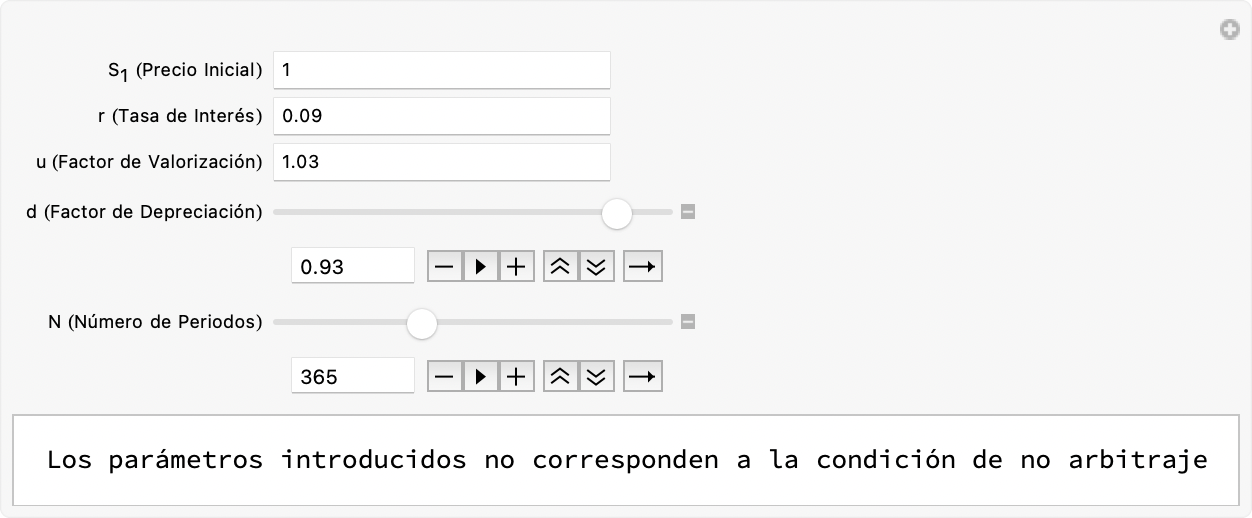
\includegraphics[width=0.45\textwidth]{sim2arb.png}
    \caption{Mensaje de error cuando se introducen parámetros que no corresponden con la condición de no arbitraje.}
    \label{fig:sim2arb}
\end{figure}

\item \emph{Elabore un programa de computadora que simule un camino aleatorio simétrico $M_n$, luego utilícelo para simular la evolución de precios dada por la fórmula:}

\begin{align*}
    S_n = e^{\sigma M_n}\left(\frac{2}{e^\sigma + e^{-\sigma}}\right)^n.
\end{align*}

\emph{El usuario debe proporcionar el parámetro $\sigma$.}

\medskip

\textbf{\textit{Sol.}} Se escribió en \texttt{Wolfram Mathematica 12.1} la siguiente función que genera contenido dinámico

\begin{doublespace}
\noindent\(\pmb{\text{Manipulate}[M=\{0\};\text{SeedRandom}[2248];}\\
\pmb{\text{For}[t=1,t<T,t\text{++},\text{ran}=\text{RandomVariate}[\text{BernoulliDistribution}[0.5]];}\\
\pmb{\text{If}[\text{ran}==1,\text{AppendTo}[M,M[[-1]]+1],\text{AppendTo}[M,M[[-1]]-1]]];}\\
\pmb{S=\text{Table}\left[e^{\sigma  M[[n]]}\left(\frac{2}{e^{\sigma }+e^{-\sigma }}\right)^n,\{n,1,T\}\right];}\\
\pmb{\text{ListLinePlot}\left[S,\text{Axes}\to \text{False},\text{Frame}\to \text{True},\text{FrameLabel}\to \left\{\text{{``}Periodo (n){''}},\text{``Precio
(}S_n\text{)''}\right\},\right.}\\
\pmb{\left.\text{ImageSize}\to \text{Full},\text{PlotRange}\to \text{All}\right],}\\
\pmb{\{\{\sigma ,0.5,\text{{``}$\sigma ${''}}\}\},\{\{T,10,\text{{``}N (N{\' u}mero de Periodos){''}}\},10,1000,1\},\text{TrackedSymbols}:\to \{\sigma ,T\}]}\)
\end{doublespace}

cuyo resultado es una ventana que permite modificar todos los parámetros y genera la gráfica resultante de dicho proceso como puede observarse en la figura \ref{fig:sim3}

\begin{figure}[h!]
    \centering
    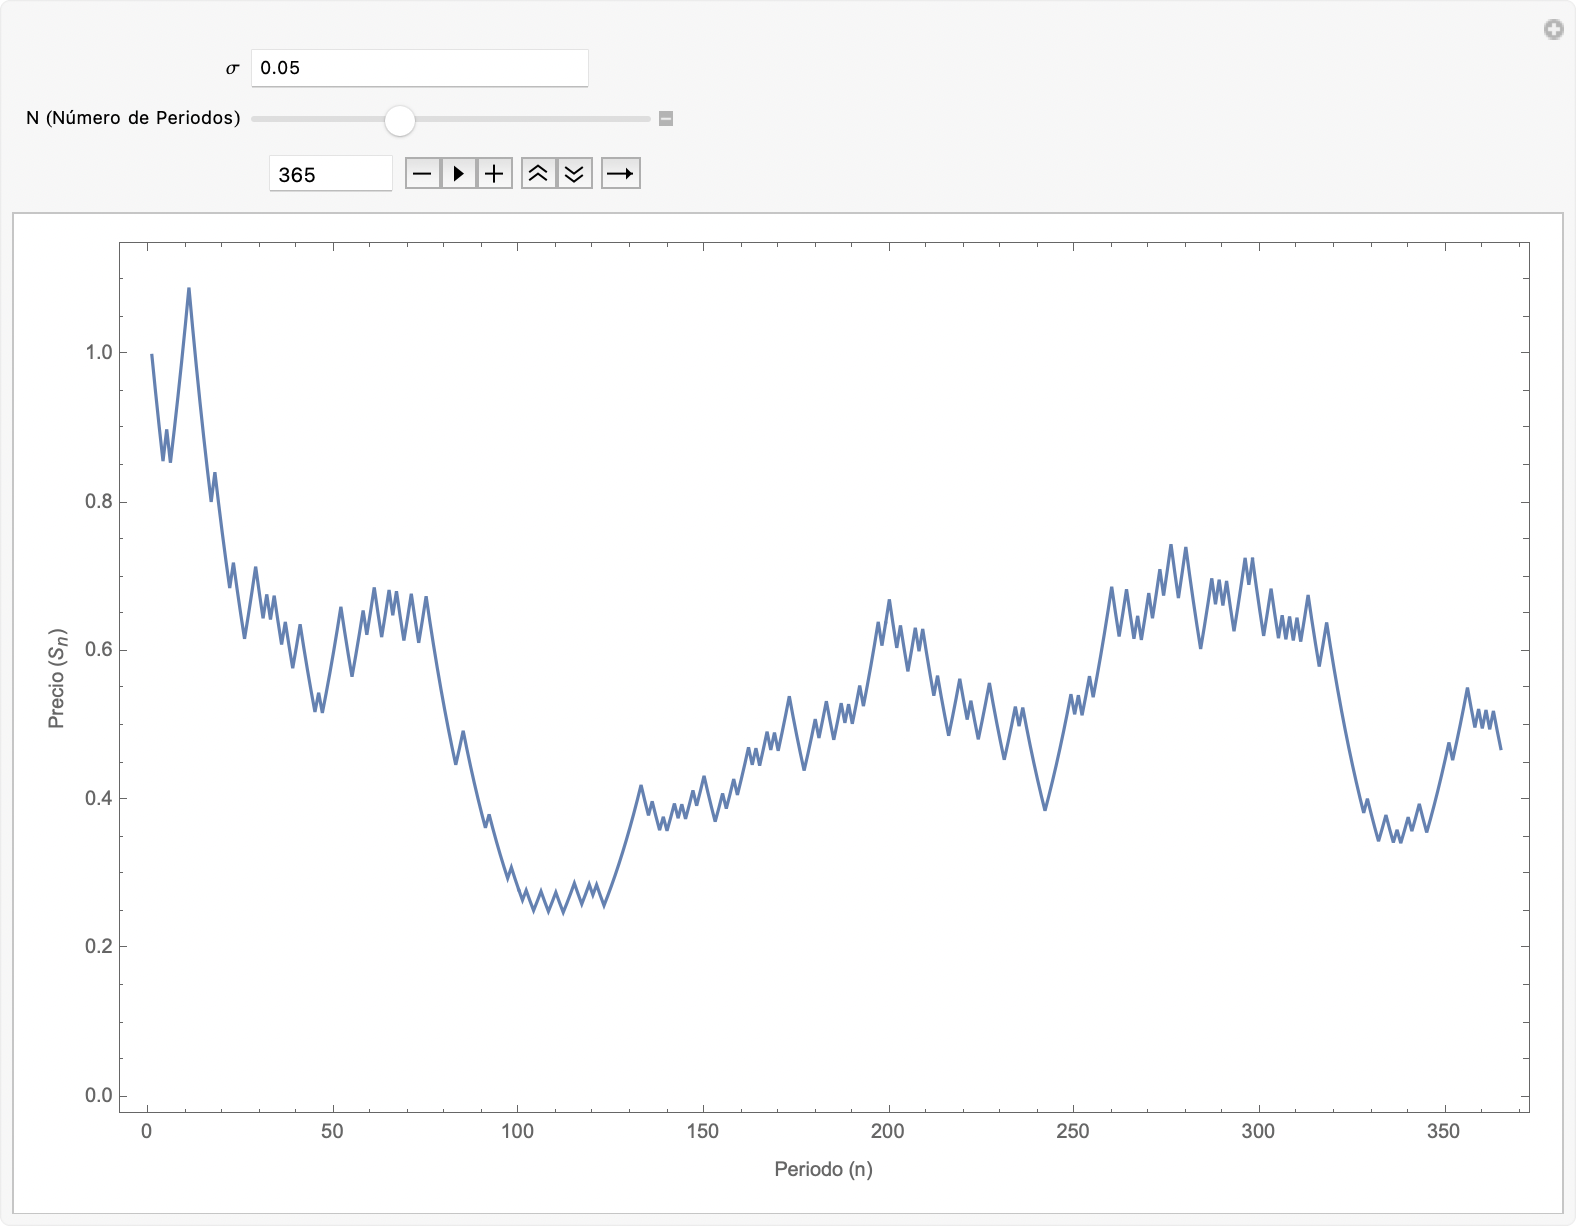
\includegraphics[width=0.5\textwidth]{sim3.png}
    \caption{Visualización del modelo de caminata aleatoria simétrica. Puede verse cómo los distintos parámetros son modificables por el usuario así como la gráfica que se genera.}
    \label{fig:sim3}
\end{figure}

\newpage

\item \emph{Repita el ejercicio anterior para un caso general que admita caminos aleatorios no simétricos (deriva hacia arriba y hacia abajo) donde el usuario debe dar las probabilidades de ascenso y descenso.}

\medskip

\textbf{\textit{Sol.}} Se escribió en \texttt{Wolfram Mathematica 12.1} la siguiente función que genera contenido dinámico

\begin{doublespace}
\noindent\(\pmb{\text{Manipulate}[M=\{0\};\text{SeedRandom}[2248];}\\
\pmb{\text{For}[t=1,t<T,t\text{++},\text{ran}=\text{RandomVariate}[\text{BernoulliDistribution}[p]];}\\
\pmb{\text{If}[\text{ran}==1,\text{AppendTo}[M,M[[-1]]+1],\text{AppendTo}[M,M[[-1]]-1]]];}\\
\pmb{S=\text{Table}\left[e^{\sigma  M[[n]]}\left(\frac{2}{e^{\sigma }+e^{-\sigma }}\right)^n,\{n,1,T\}\right];}\\
\pmb{\text{ListLinePlot}\left[S,\text{Axes}\to \text{False},\text{Frame}\to \text{True},\text{FrameLabel}\to \left\{\text{{``}Periodo (n){''}},\text{``Precio
(}S_n\text{)''}\right\},\right.}\\
\pmb{\left.\text{ImageSize}\to \text{Full},\text{PlotRange}\to \text{All}\right],}\\
\pmb{\{\{p,0.5,\text{{``}p (Probabilidad de Ascenso){''}}\},0.01,0.99\},\{\{\sigma ,0.5,\text{{``}$\sigma ${''}}\}\},}\\
\pmb{\{\{T,10,\text{{``}N (N{\' u}mero
de Periodos){''}}\},10,1000,1\},\text{TrackedSymbols}:\to \{p,\sigma ,T\}]}\)
\end{doublespace}

cuyo resultado es una ventana que permite modificar todos los parámetros y genera la gráfica resultante de dicho proceso como puede observarse en la figura \ref{fig:sim4}

\begin{figure}[h!]
    \centering
    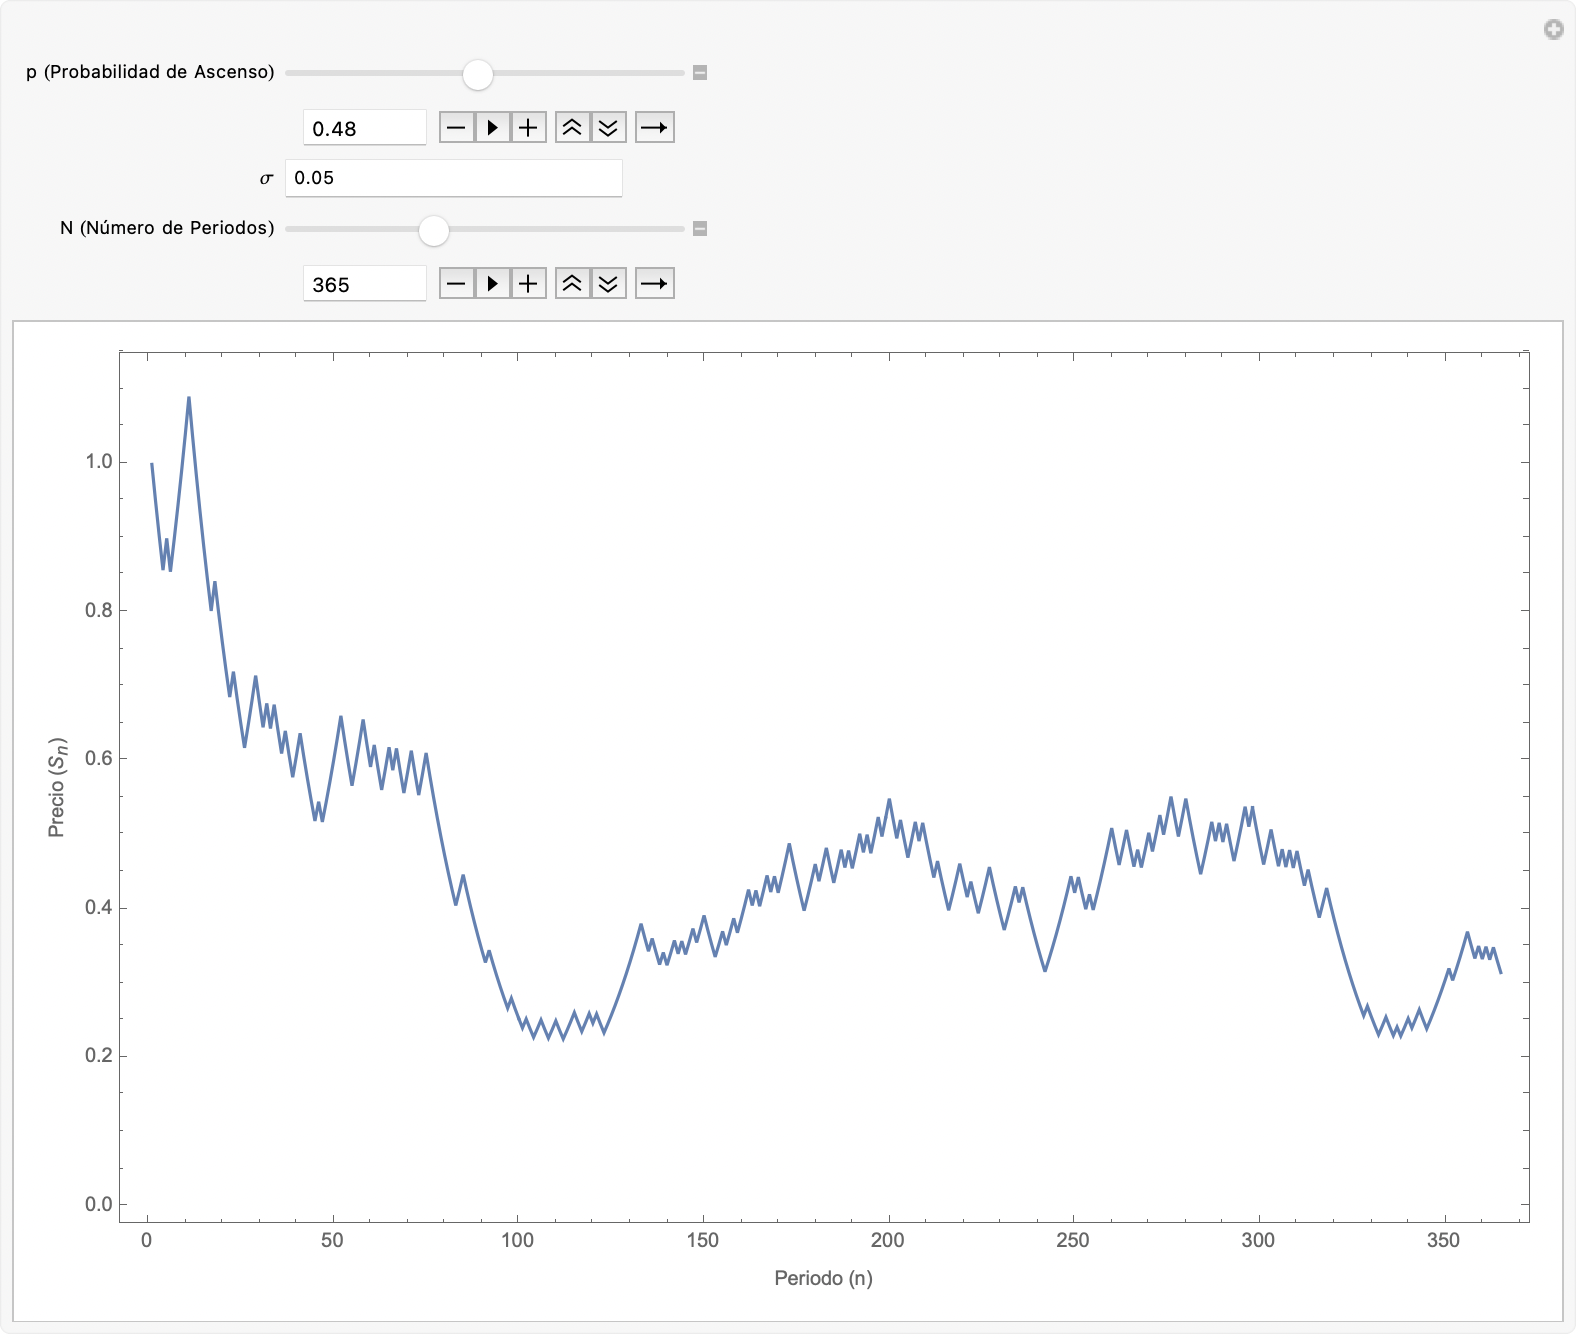
\includegraphics[width=0.5\textwidth]{sim4.png}
    \caption{Visualización del modelo de caminata aleatoria no simétrica. Puede verse cómo los distintos parámetros son modificables por el usuario así como la gráfica que se genera.}
    \label{fig:sim4}
\end{figure}

\item \emph{Utilizando los algoritmos anteriores proponga un módulo que le permita simular tiempos de parada para modelos binomiales con periodos finitos y tiempos de alcance para valores prefijados en modelos basados en caminos aleatorios.}

\medskip

\textbf{\textit{Sol.}} 

\item \emph{Realice más de 10 simulaciones para cada caso y describa sus observaciones. En especial describa las diferencias observadas entre los modelos del punto 1) y del punto 3).}

\medskip

\textbf{\textit{Sol.}} Se realizaron varias simulaciones con cada uno de los módulos, no todas las cuales vale la pena poner acá pues ocuparían mucho espacio, sin embargo son particularmente interesantes algunas observaciones.

\begin{itemize}

\item Como era de esperarse, los módulos desarrollados para los ejercicios \emph{(1)} y \emph{(2)} generan el mismo comportamiento siempre que se introduzcan la probabilidad y la tasa de interés correctas (i.e., tales que la probabilidad de riesgo neutral calculada con dicha tasa de interés sea la misma probabilidad introducida directamente en \emph{(1)}), un ejemplo tal puede verse en la figura \ref{fig:comp1-2}.

\begin{figure}[h!]
    \centering
    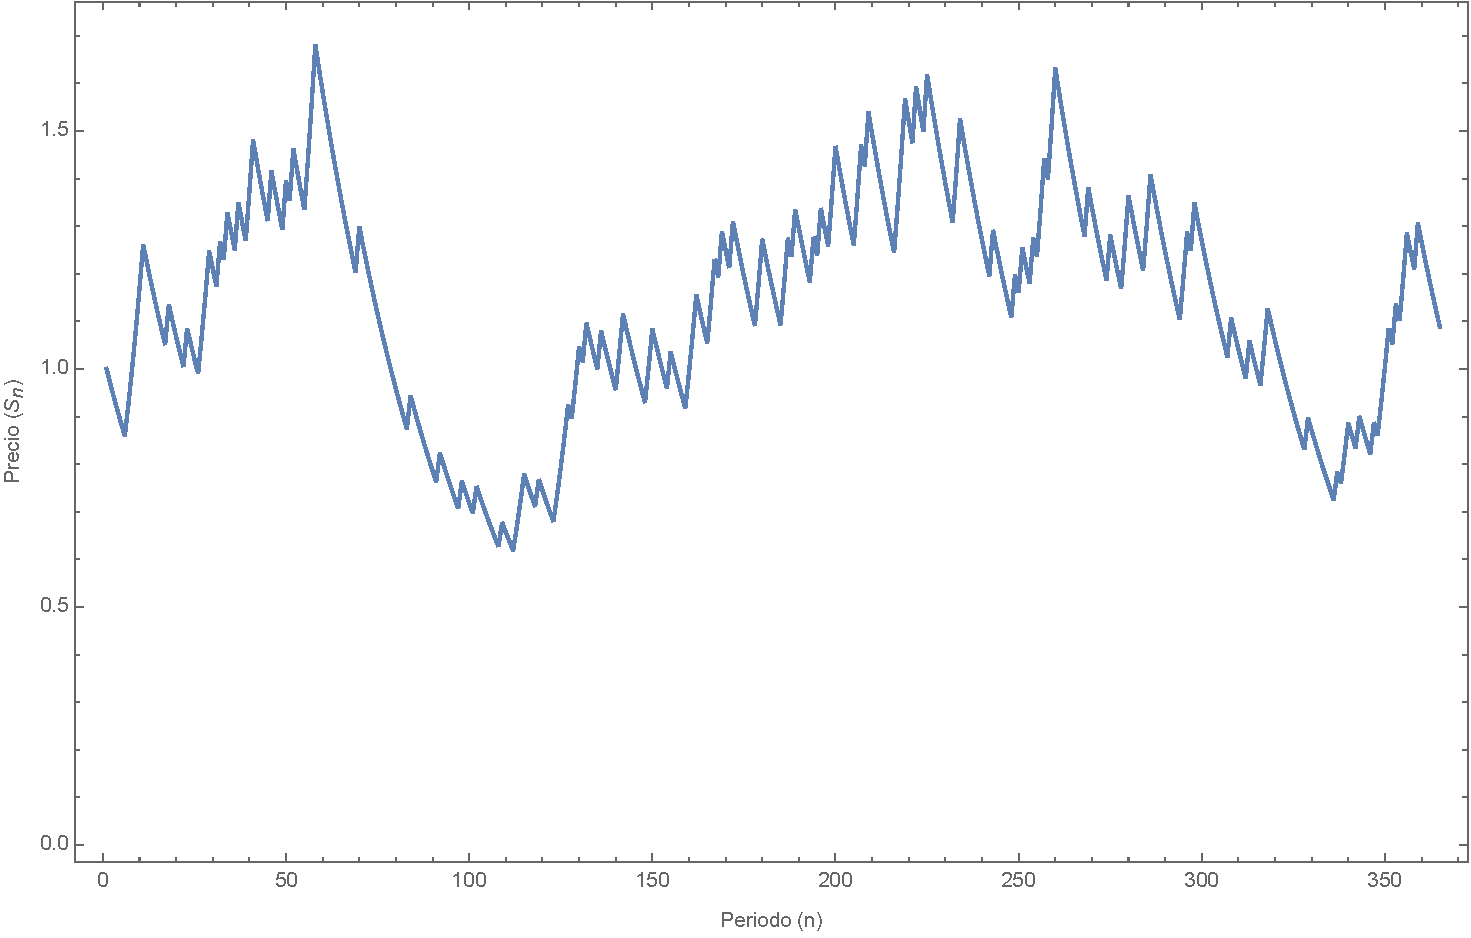
\includegraphics[width=0.7\textwidth]{comp1-2.pdf}
    \caption{Comportamiento para $365$ periodos generado tanto por el primer como por el segundo módulo usando $u = 1.08, d = 0.97$ en ambos y $p = 0.3$ en el primero y $r = 0.0018$ en el segundo.}
    \label{fig:comp1-2}
\end{figure}

\item El comportamiento generado por el módulo desarrollado para el ejercicio \emph{(3)}, el cual se basa en una caminata aleatoria simétrica, es exactamente el comportamiento que se observa en el modelo de árbol binomial (primer módulo) cuando la probabilidad de valorización es $0.5$ y cuando se toma $u = 1 + \sigma, d = 1 - \sigma$, un ejemplo de esto puede verse en la figura \ref{fig:comp1-3}.

\begin{figure}[h!]
    \centering
    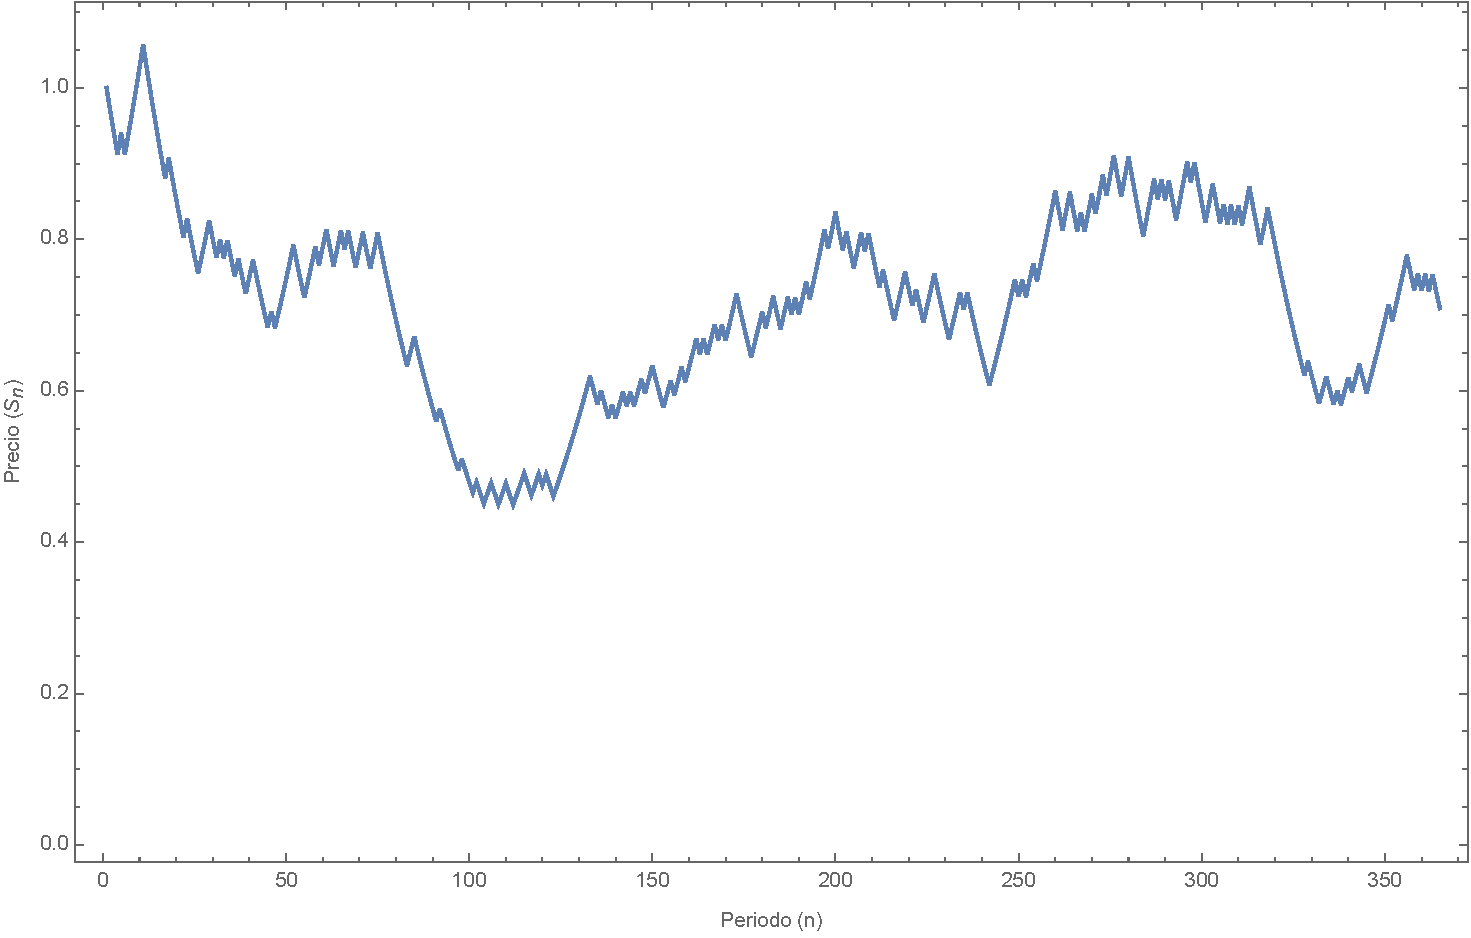
\includegraphics[width=0.7\textwidth]{comp1-3.pdf}
    \caption{Comportamiento para $365$ periodos generado tanto por el primer como por el tercer módulo usando $u = 1.03, d = 0.97, p = 0.5$ en el primero y $\sigma = 0.03$ en el tercero.}
    \label{fig:comp1-3}
\end{figure}

\item El comportamiento generado por el módulo desarrollado para el ejercicio \emph{(4)}, el cual se basa en una caminata aleatoria no simétrica, es exactamente el comportamiento que se observa en el modelo de árbol binomial (primer módulo) cuando la probabilidad de valorización es igual a la probabilidad de ascenso y cuando se toma $u = 1 + \sigma, d = 1 - \sigma$, un ejemplo de esto puede verse en la figura \ref{fig:comp1-4}.

\begin{figure}[h!]
    \centering
    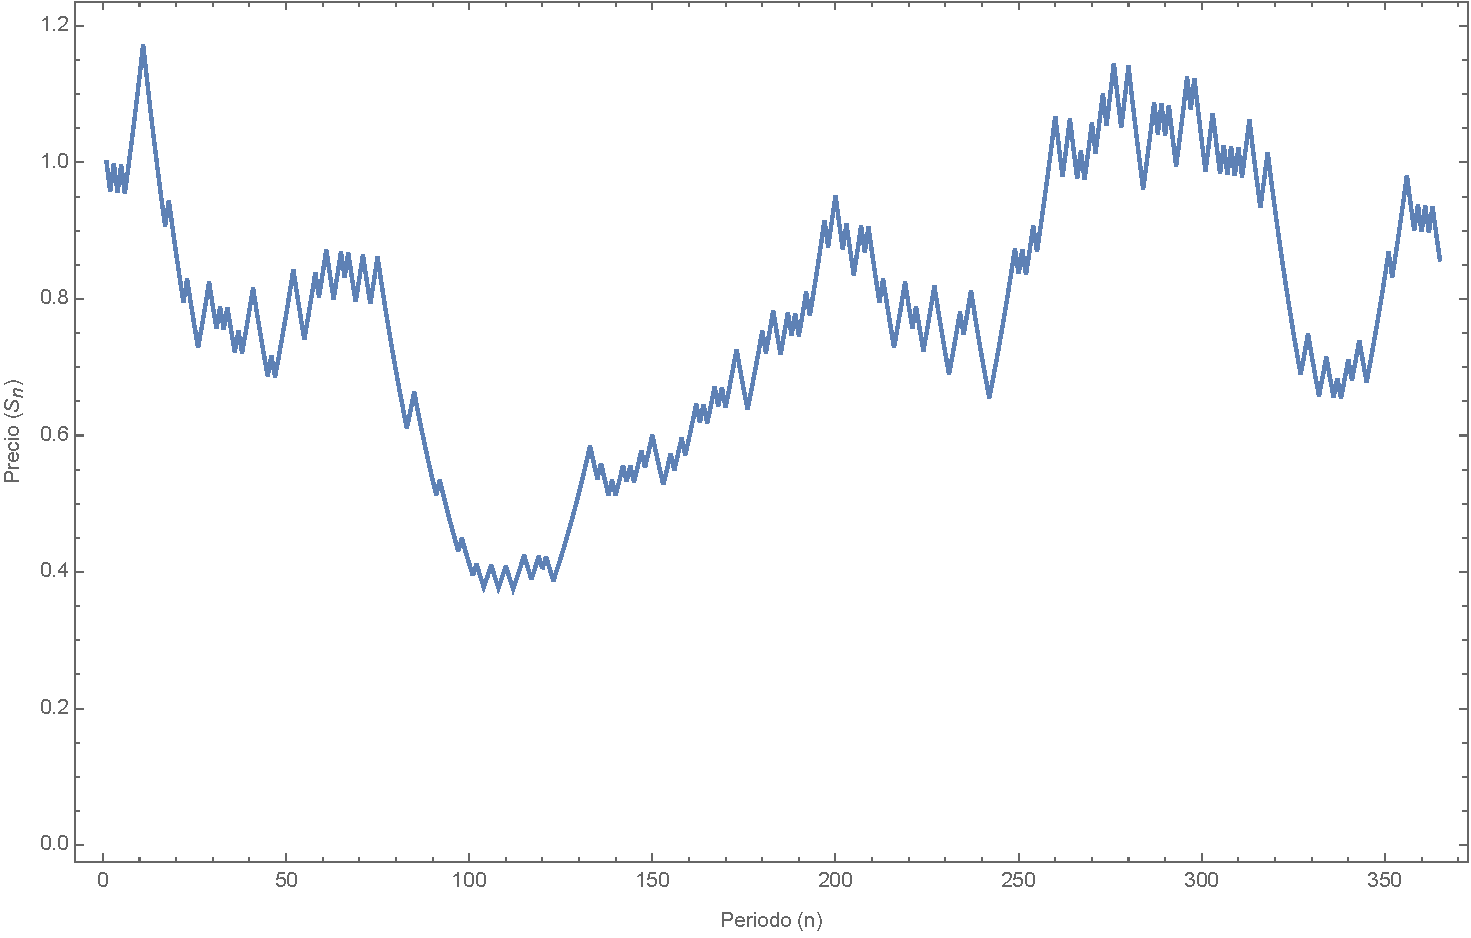
\includegraphics[width=0.7\textwidth]{comp1-4.pdf}
    \caption{Comportamiento para $365$ periodos generado tanto por el primer como por el cuarto módulo usando $u = 1.042, d = 0.958, p = 0.51$ en el primero y $\sigma = 0.042, p = 0.51$ en el cuarto.}
    \label{fig:comp1-4}
\end{figure}

\end{itemize}

\newpage

\item \emph{Desarrolle un módulo que le permita al usuario introducir una gestión del portafolio tipo delta para visualizar procesos de capitalización regidos por la fórmula}

\begin{align*}
    X_{n+1} = \Delta_nS_{n+1} + (1 + r)(X_n - \Delta_nS_n).
\end{align*}

\emph{En otras palabras, realice un algoritmo que (con base en la simulación para la serie de precios $S_n$) le permita al usuario ingresar las operaciones $\Delta_n$ para obtener la serie de capital acumulado $X_n$. Su algoritmo debe permitirle al usuario saber cuándo debe apalancar recursos, en otras palabras debe alertar aquellas situaciones en que $Xn - \Delta_nS_n < 0$.}

\medskip

\textbf{\textit{Sol.}} Se escribió en \texttt{Wolfram Mathematica 12.1} la siguiente función que genera contenido dinámico

\begin{doublespace}
\noindent\(\pmb{\text{Manipulate}[T=\text{Length}[\Delta ];\text{SeedRandom}[2248];}\\
\pmb{\text{If}[d<1+r<u,S=\{\text{S1}\};p=\frac{1+r-d}{u-d};}\\
\pmb{\text{For}[n=1,n<T,n\text{++},\text{ran}=\text{RandomVariate}[\text{BernoulliDistribution}[p]];}\\
\pmb{\text{If}[\text{ran}==1,\text{AppendTo}[S,S[[-1]]u],\text{AppendTo}[S,S[[-1]]d]]],}\\
\pmb{\text{Catch}[\text{Throw}[\text{{``}Los par{\' a}metros introducidos
no corresponden a la condici{\' o}n de no arbitraje{''}}]]];}\\
\pmb{X=\{S[[1]]\};\text{For}[n=1,n<T,n\text{++},\text{If}[X[[n]]-\Delta [[n]]S[[n]]<0,\text{Echo}[n,\text{{``}Apalancar en {''}}];}\\
\pmb{\text{AppendTo}[X,\Delta [[n]]S[[n+1]]+(1+r)(X[[n]]-\Delta [[n]]S[[n]])],}\\
\pmb{\text{AppendTo}[X,\Delta [[n]]S[[n+1]]+(1+r)(X[[n]]-\Delta [[n]]S[[n]])]]];}\\
\pmb{\text{ListLinePlot}\left[X,\text{Axes}\to \text{False},\text{Frame}\to \text{True},\text{FrameLabel}\to \left\{\text{{``}Periodo (n){''}},\text{``Capital
Acumulado (}X_n\text{)''}\right\},\right.}\\
\pmb{\left.\text{ImageSize}\to \text{Full},\text{PlotRange}\to \text{All}\right],}\\
\pmb{\left\{\left\{\text{S1},4,\text{``}S_1\text{ (Precio Inicial)''}\right\}\right\},\{\{r,0.05,\text{{``}r (Tasa de Inter{\' e}s){''}}\}\},\{\{u,2,\text{{``}u
(Factor de Valorizaci{\' o}n){''}}\}\},}\\
\pmb{\left\{\left\{d,\frac{1}{u},\text{{``}d (Factor de Depreciaci{\' o}n){''}}\right\},0,u\right\},\left.\left\{\left\{\Delta ,\{0.5,0.4,0.3,0.6,0.7,0.8\},\right.\right.\right.}\\
\pmb{\left.\left.\left.\text{``$\Delta $ (Operaciones }\Delta _n\text{, introducir entre corchetes
y separ{\' a}ndo los n{\' u}meros por comas)''}\right\}\right\},\right.}\\
\pmb{\left.\text{TrackedSymbols}:\to \{\text{S1},r,\sigma ,\Delta \}\right]}\)
\end{doublespace}

cuyo resultado es una ventana que permite modificar todos los parámetros y genera la gráfica resultante de dicho proceso, además de que imprime mensajes indicando los periodos en los que se debe apalancar recursos, como puede observarse en la figura \ref{fig:sim7}

\begin{figure}[h!]
    \centering
    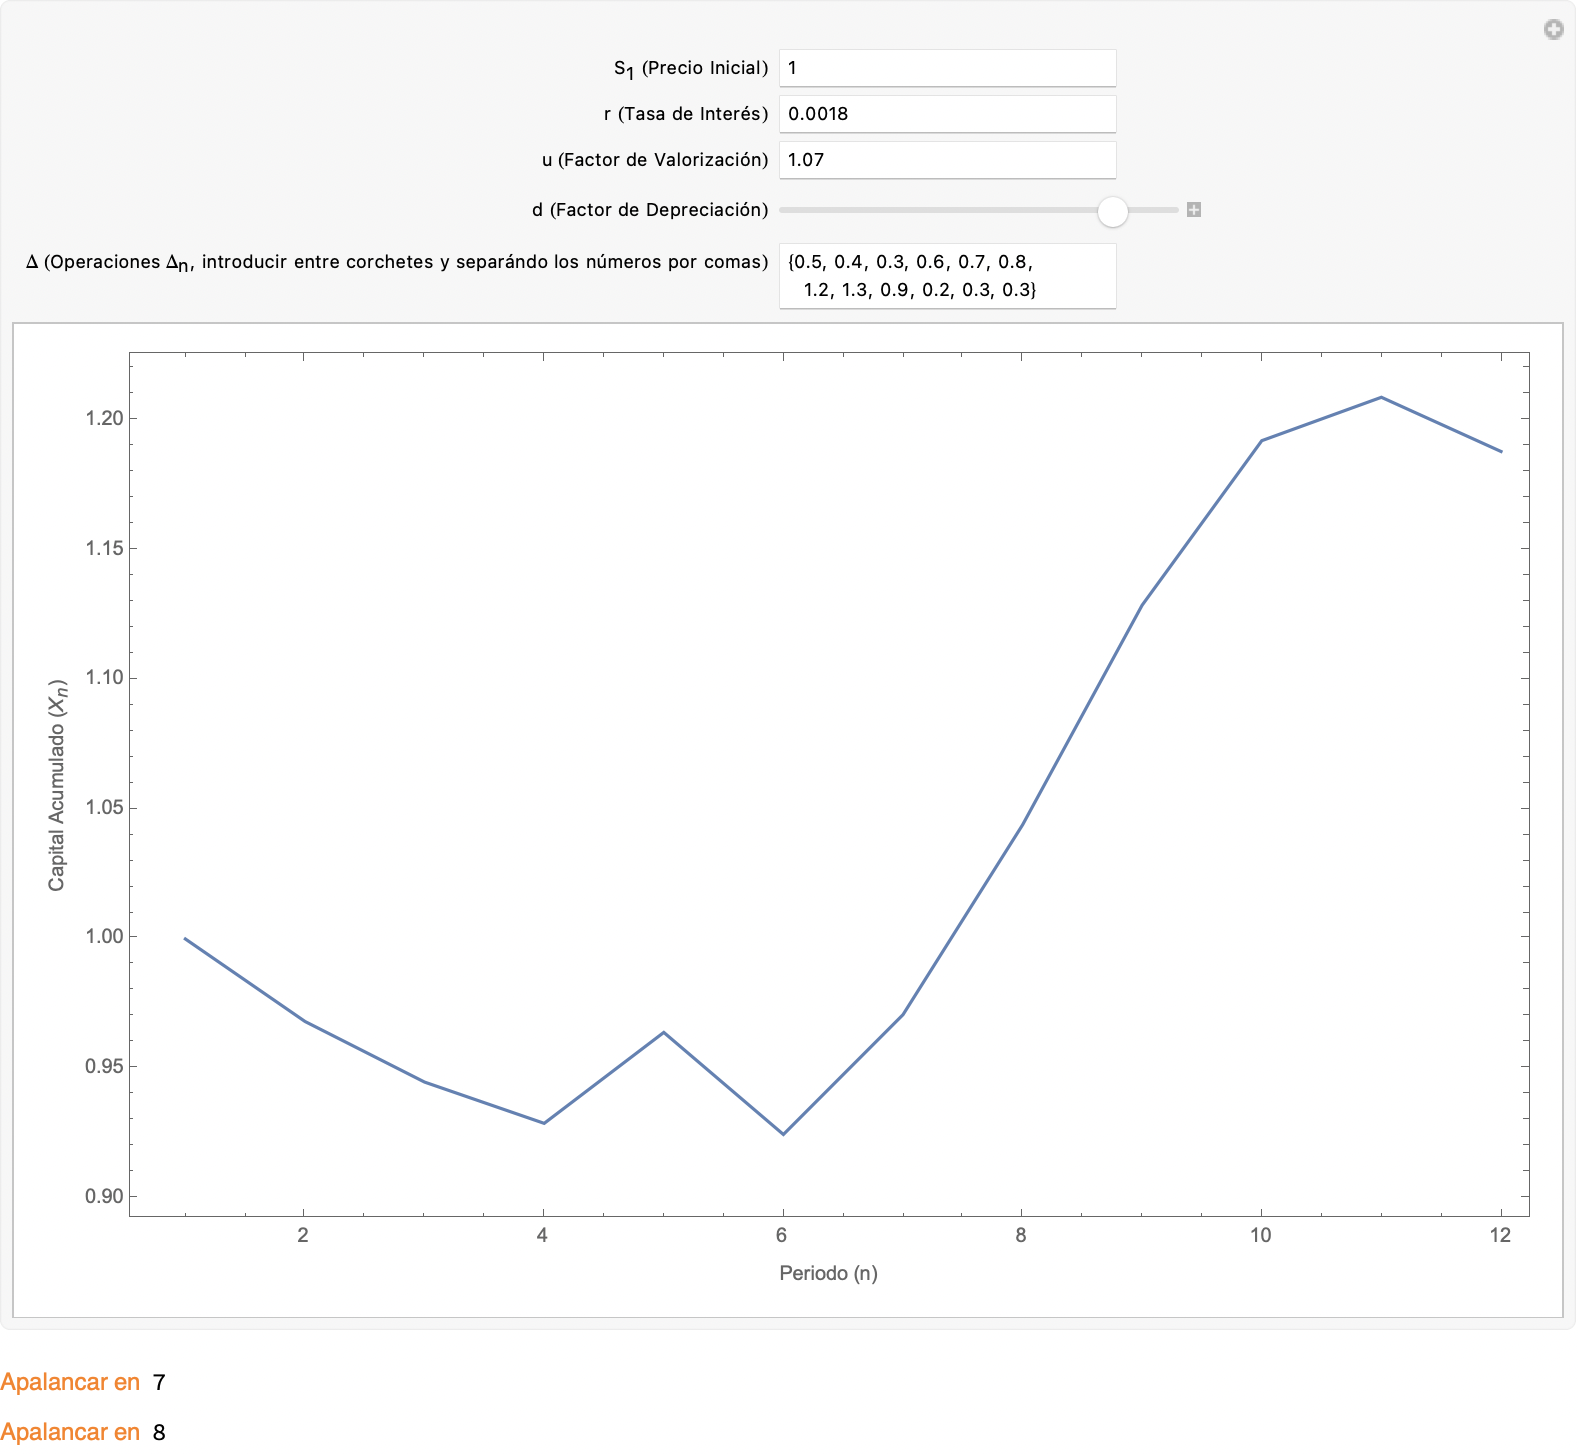
\includegraphics[width=0.5\textwidth]{sim7.png}
    \caption{Visualización de gestión de portafolio \emph{delta}. Puede verse cómo los distintos parámetros son modificables por el usuario así como la gráfica que se genera y los mensajes de alerta.}
    \label{fig:sim7}
\end{figure}

\item \emph{Elabore un módulo que reciba la función de pagos de un derivado tipo europeo
$V_N = V_N(\omega_1,\dots,\omega_N)$, los parámetros de un modelo binomial y que devuelva la valoración del derivado en los periodos intermedios $n = 0,\dots,N-1$.}

\textbf{\textit{Sol.}} Se escribió en \texttt{Wolfram Mathematica 12.1} la siguiente función que genera contenido dinámico

\begin{doublespace}
\noindent\(\pmb{\text{Manipulate}[V=\{\text{VN}\};\text{SeedRandom}[2248];}\\
\pmb{\text{For}\left[i=1,i<T,i\text{++},\text{PrependTo}\left[V,\frac{\text{Expectation}\left[V[[1]],n\unicode{f3d2}\text{BinomialDistribution}\left[T-i,\frac{1+r-d}{u-d}\right]\right]}{1+r}\right]\right];}\\
\pmb{\text{ListLinePlot}[V,\text{Axes}\to \text{False},\text{Frame}\to \text{True},\text{FrameLabel}\to \{\text{{``}Periodo ($n$){''}},\text{{``}Precio ($V_n$){''}}\},}\\
\pmb{\text{ImageSize}\to
\text{Full},\text{PlotRange}\to \text{All}],\left\{\left\{\text{VN},4 u^nd^{T-n},``V_N\text{ (Funci{\' o}n de Pagos)''}\right\}\right\},}\\
\pmb{\{\{u,2,\text{{``}u (Factor de Valorizaci{\' o}n){''}}\}\},\left\{\left\{d,\frac{1}{u},\text{{``}d (Factor de Depreciaci{\' o}n){''}}\right\},0,u\right\},}\\
\pmb{\{\{r,0.05,\text{{``}r
(Tasa de Inter{\' e}s){''}}\}\},\{\{T,10,\text{{``}N{\' u}mero de Periodos{''}}\},10,1000,1\},\text{TrackedSymbols}:\to \{\text{VN},u,d,r,T\}]}\)
\end{doublespace}

cuyo resultado es una ventana que permite modificar todos los parámetros y genera la gráfica resultante de dicho proceso como puede observarse en la figura \ref{fig:sim8}

\begin{figure}[h!]
    \centering
    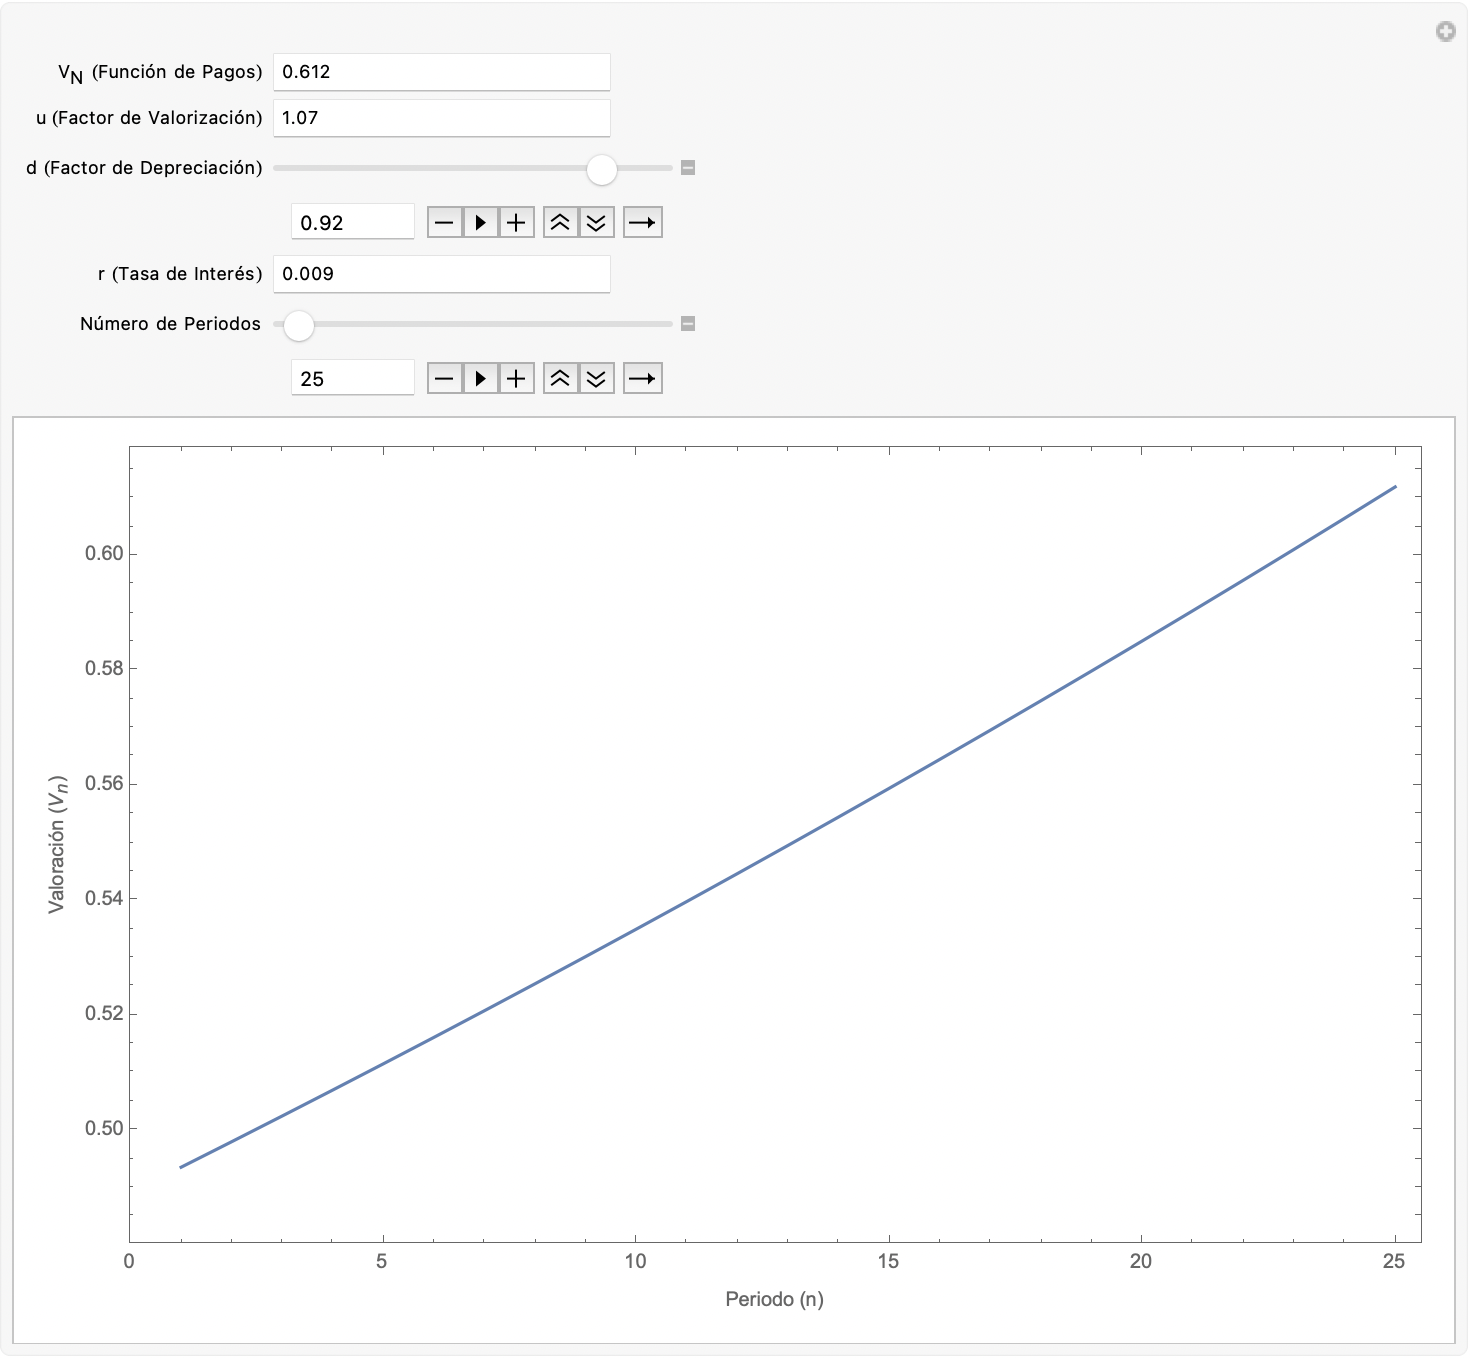
\includegraphics[width=0.5\textwidth]{sim8.png}
    \caption{Visualización de valoración de un derivado dada una función de pagos. Puede verse cómo los distintos parámetros son modificables por el usuario así como la gráfica que se genera.}
    \label{fig:sim8}
\end{figure}

\newpage

\item \emph{Complete el punto anterior para que el módulo correspondiente proporcione al usuario la operación delta que replica el derivado en cuestión. Esta es:}

\begin{align*}
    \Delta_n(\omega_1,\dots,\omega_n) = \frac{V_{n+1}(\omega_1,\dots,\omega_nu) - V_{n+1}(\omega_1,\dots,\omega_nd)}{S_{n+1}(\omega_1,\dots,\omega_nu) - S_{n+1}(\omega_1,\dots,\omega_nd)}
\end{align*}

\emph{Introduzca estos datos en el punto 7) para verificar que efectivamente replica el derivado.}

\textbf{\textit{Sol.}} Se le añadió al módulo anterior la instrucción

\begin{doublespace}
\noindent\(\pmb{\text{$\Delta $rep}=\text{Table}\left[\frac{uV[[i]]-dV[[i]]}{uS[[i]]-dS[[i]]},\{i,1,T\}\right]}\)
\end{doublespace}

que guarda en una variable \pmb{$\Delta$rep} la estrategia de replicación, la cual al introducirse en el módulo del ejercicio \emph{(7)} efectivamente replica el derivado, como puede verse en las figuras \ref{fig:org} y \ref{fig:rep}.

\begin{figure}[h!]
    \centering
    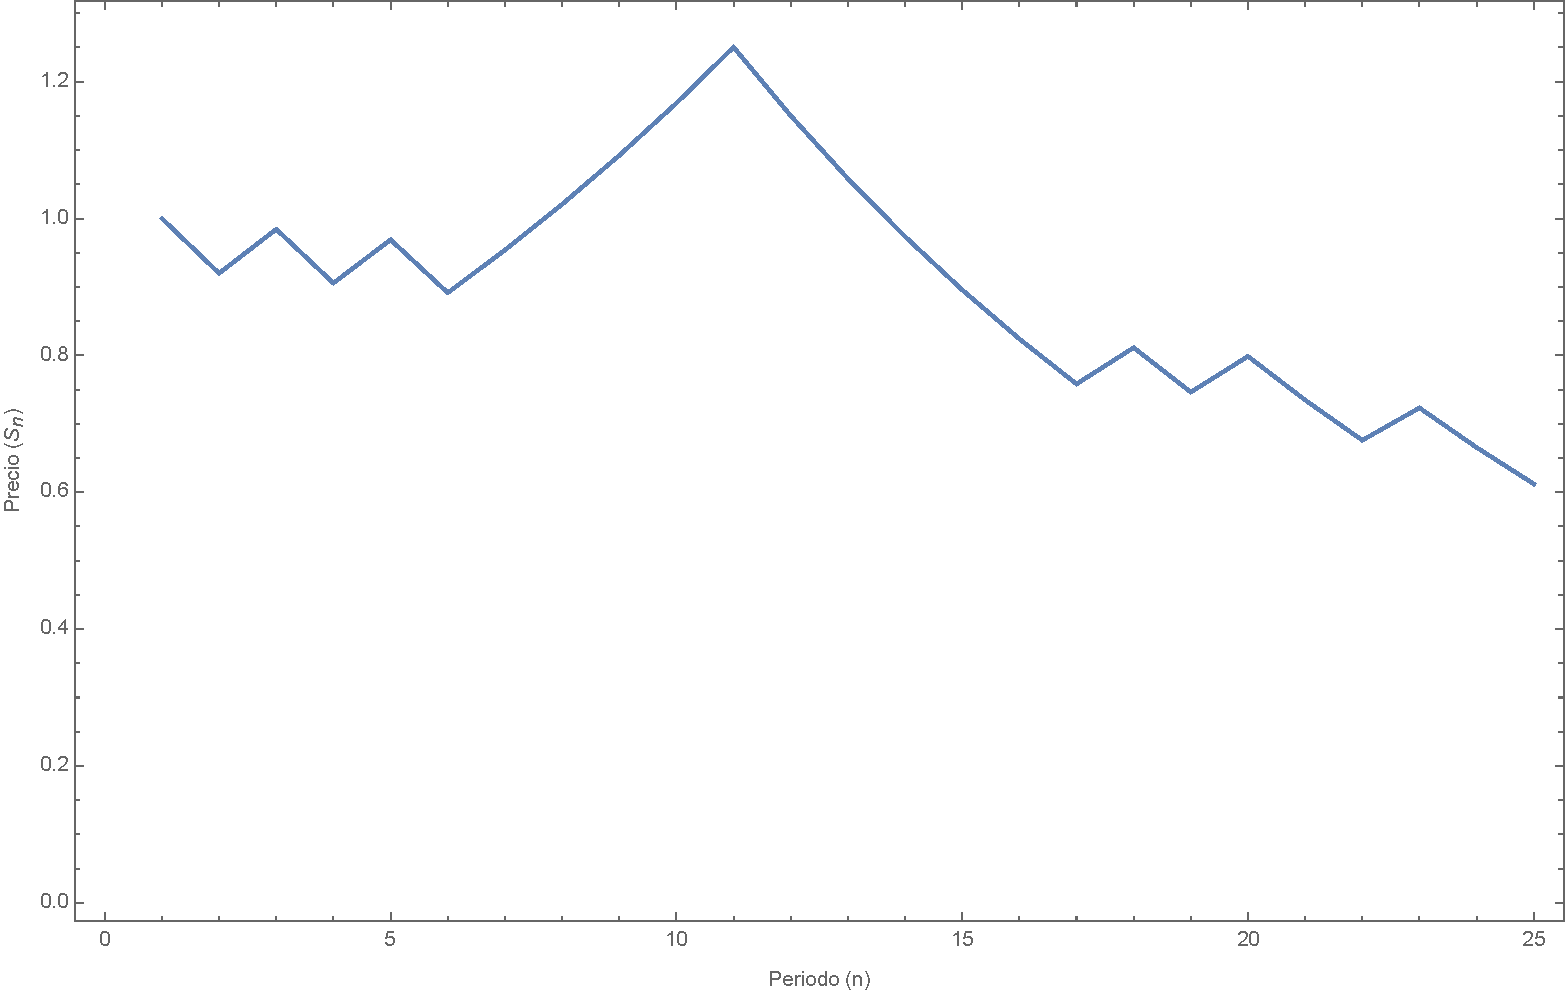
\includegraphics[width=0.5\textwidth]{org.pdf}
    \caption{Comportamiento del derivado según simulación con módulo de ejercicio (2).}
    \label{fig:org}
\end{figure}

\begin{figure}[h!]
    \centering
    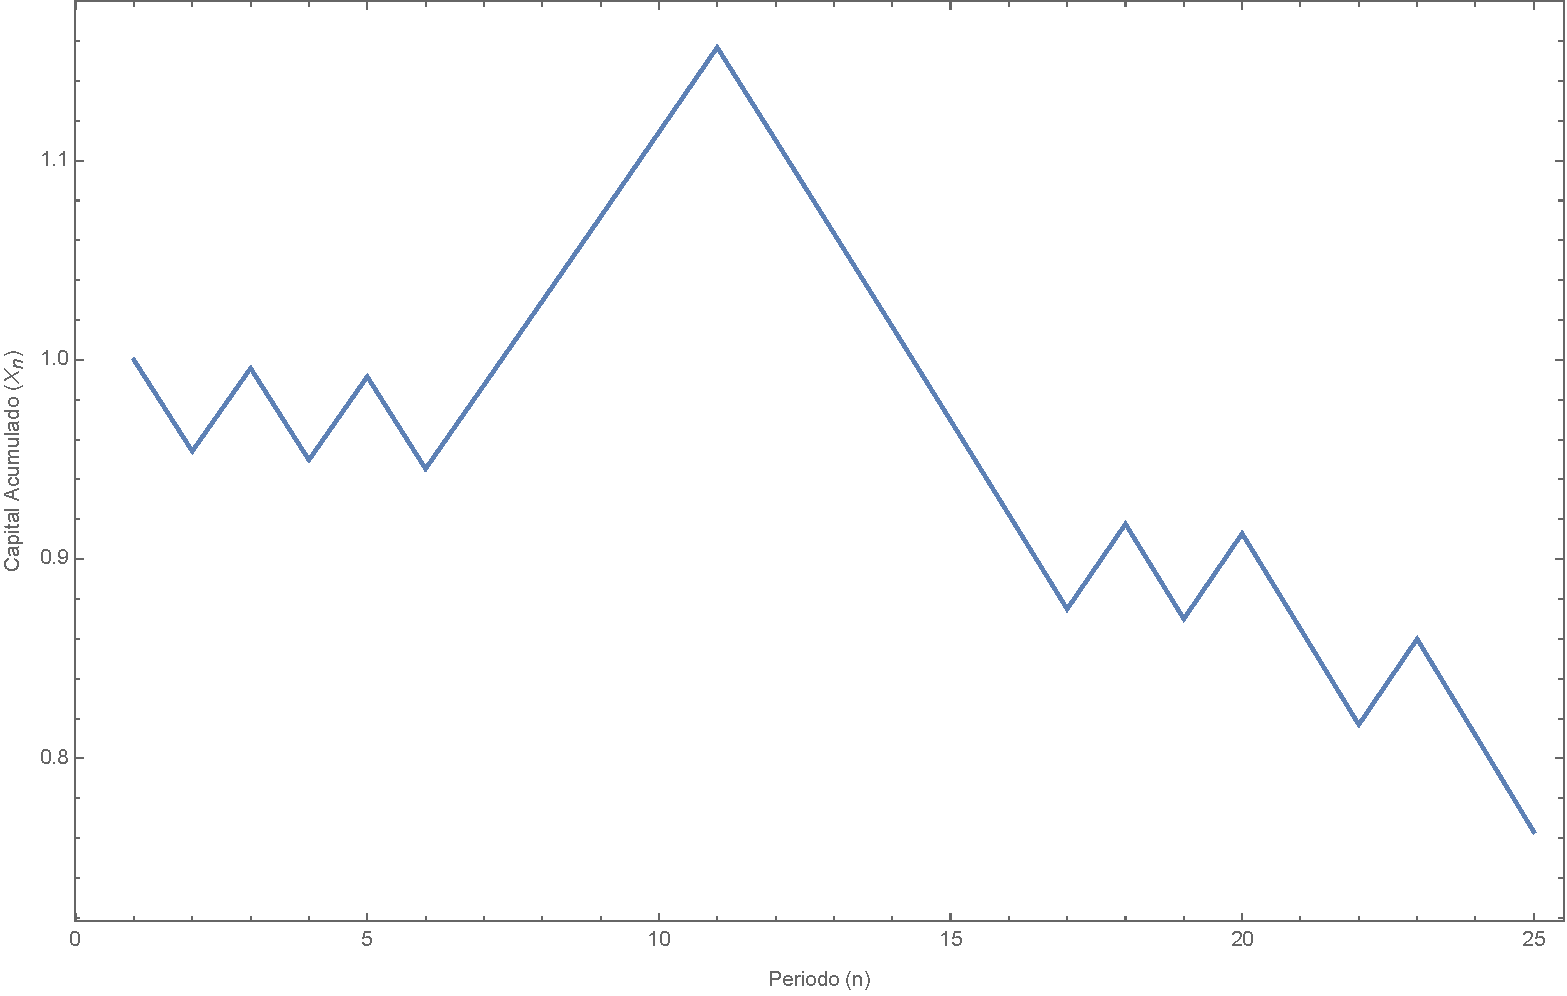
\includegraphics[width=0.5\textwidth]{rep.pdf}
    \caption{Comportamiento del portafolio \emph{delta} usando estrategia de replicación.}
    \label{fig:rep}
\end{figure}

\newpage

\item \emph{Utilice estadística descriptiva sobre varias simulaciones con los resultados del punto 1) para mostrar que $\frac{S_n}{(1 + r)^n}$ es una martingala.}

\textbf{\textit{Sol.}} Se realizaron varias simulaciones usando el módulo del ejercicio \emph{(2)} para $365$ periodos y luego se calculó directamente el valor esperado de $\frac{S_{n+1}}{(1 + r)^{n+1}}$ como

\begin{align*}
    \mathbb{E}\left[\frac{S_{n+1}}{(1 + r)^{n+1}}\right] = \frac{p^*uS_n + (1 - p^*)dS_n}{(1 + r)^{n+1}},
\end{align*}

tras lo cual se calculó la media de las desviaciones entre éstos y el valor en la simulación de $\frac{S_n}{(1 + r)^n}$. Se esperaba que estas desviaciones fuesen $0$ pues para una martingala

\begin{align*}
    \mathbb{E}\left[\frac{S_{n+1}}{(1 + r)^{n+1}}\right] = \frac{S_n}{(1 + r)^n}.
\end{align*}

En efecto estas desviaciones estuvieron siempre muy cerca de $0$, en el orden de $10^{-17}$, lo cual se cree que se debe a pequeños errores en distintos puntos de los cálculos al ser éstos enteramente numéricos, por lo cual tienen una precisión máxima.

\end{enumerate}

\end{document}